% das Dokumentenformat asdf
\documentclass[a4paper, 12pt, twppages]{article}

%\usepackage[english, ngerman]{babel}  % <-- f�r deutsche arbeit

% wegen deutschen Umlauten - Details: http://www.golatex.de/usepackagelatin1inputenc-vs-usepackaget1fontenc-t7624.html
\usepackage[T1]{fontenc}
\usepackage[ansinew]{inputenc} % auf Zeichencodierung der Datei achten! In TeXnicCenter im "Speichern Unter"-Dialog 'ANSI' ausw�hlen.
%\usepackage[utf8]{inputenc} % alternative Zeichencodierung 'UTF-8'

%% IMAGE PACKAGE
\usepackage{graphicx}

%% PACKAGE FOR THE BACKGROUNDPIC
\usepackage{eso-pic}

%% PACKAGE FOR THE HEADERS AND FOOTERS
\usepackage{fancyhdr}

%% PACKAGE TO INCLUDE A PDF FILE
\usepackage{pdfpages}

%% OTHER PACKAGES
%\usepackage[numbers]{natbib}
\usepackage{hyperref}
\usepackage{enumitem}
\usepackage{caption}
\usepackage{subcaption}
\usepackage[toc,page]{appendix}
\usepackage{multirow}
\usepackage{longtable}
%\usepackage{tabularx}
\usepackage[flushleft]{threeparttable}
\usepackage{siunitx}
\usepackage{ifthen}

\urlstyle{same}

\newcommand\BackgroundPic{%
\put(0,0){%
\parbox[b][\paperheight]{\paperwidth}{%
\vfill
\centering

\includegraphics[width=\paperwidth,height=\paperheight,keepaspectratio]{template/background.pdf}%
\vfill
}}}
\setlength{\footskip}{68pt}
\fancyhf{}% Clear all headers/footers
\renewcommand{\headrulewidth}{0pt}% No header rule
\renewcommand{\footrulewidth}{0pt}% No footer rule
\fancyfoot[L]{\hspace*{-16mm}
\includegraphics[scale=0.3]{template/logoDepartment.pdf}}

\begin{document}


\includepdf[pages={1}]{template/scan-of-declaration-of-authorship.pdf}
\pagebreak

\AddToShipoutPicture*{\BackgroundPic}
\thispagestyle{fancy}

{\vspace{2cm}~}
{\vspace{2cm}}

%% SELECT BACHELOR OR MASTER THESIS
{\noindent\large Master Thesis}


\vspace{1cm}

%% WRITE THE TITLE OF YOUR WORK
{\noindent\huge\textbf{Collaboration networks in open-source software development}}

\bigskip

%% WRITE YOUR NAME, date of birth, Student ID
{\noindent\LARGE Jozsef Csepanyi}

%% WRITE YOUR date of birth, Student ID
\bigskip
{\noindent\small Date of Birth: 06.09.1996}\newline
{\noindent\small Student ID: 11927479}

\bigskip
{\vspace{2cm}}
{\noindent\large {\bf Subject Area:} Information Systems}

%% WRITE YOUR Studienkennzahl
\bigskip
{\noindent\large {\bf Studienkennzahl:} h11927479}

\bigskip


%% WRITE THE NAME OF YOUR SUPERVISOR
{\noindent\large {\bf Supervisor:} Johannes Wachs}

\bigskip

%% WRITE THE DATAE OF SUBMISSION
{\noindent\large {\bf Date of Submission:} 02. April 2021}

\bigskip\bigskip\bigskip\bigskip\bigskip\bigskip

{\em\noindent Department of Information Systems and Operations, Vienna University of
Economics and Business, Welthandelsplatz 1, 1020 Vienna, Austria
}


\pagebreak
\tableofcontents
\pagebreak
\listoffigures
\pagebreak
\listoftables
\pagebreak

\setlength{\footskip}{30pt}

\begin{abstract}

Aenean commodo ligula eget dolor. Aenean massa. Cum sociis natoque penatibus et magnis dis parturient montes, nascetur ridiculus mus. Donec quam felis, ultricies nec, pellentesque eu, pretium quis, sem. Nulla consequat massa quis enim. Donec pede justo, fringilla vel, aliquet nec, vulputate eget, arcu. In enim justo, rhoncus ut, imperdiet a, venenatis vitae, justo. Nullam dictum felis eu pede mollis pretium. Integer tincidunt. Cras dapibus. Vivamus elementum semper nisi. Aenean vulputate eleifend tellus. Aenean leo ligula, porttitor eu, consequat vitae, eleifend ac, enim. Aliquam lorem ante, dapibus in, viverra quis, feugiat a, tellus.\dots
\end{abstract}

\pagebreak

\thepage
\section{Introduction}

%- No collocation
%- Enterprise support
%- Version control, issue tracking

In recent years open source software solutions have become widely popular and frequently used in both scientific and enterprise use, which can be attributed to a number of factors, most importantly the ease of development and deployment of IT projects, improved cybersecurity and enhanced scalability \cite{pwcLeadingBenefitsOpensource2016}. This increases the contribution to open source projects from enterprises and individuals alike. Due to its nature, open source software projects are driven by community contributions, and depend heavily on active participation in all phases of the project. \\

Software development in a corporate environment usually follows a strict hierarchial structure, where each participant is given a precise position and responsibility, like project manager, scrum master, senior or junior developer, and employees do not tend to work outside of their assigned tasks and territories. The main purpose of maintaining software development structures is for the company to ensure that the outcome of the project is in accordance with the business objective, adheres to the pre-set quality criteria and it is completed in a given timeframe; in other words to asses the risks associated with the business objective of the software project \cite{surekaUsingSocialNetwork2011}. This is achieved by breaking down the developed software into smaller, less complex components, and grouping the developers into managable teams, where the communication is moderated between teams \cite{birdLatentSocialStructure2008}. \\

% Open-source software development properties
As opposed to commercial software development, Free/Libre Open Source Software (FLOSS) projects usually do not follow an organizational hierarchy, and are usually self-organizing and dynamic \cite{birdLatentSocialStructure2008}. Issues, bugs and progress are tracked openly, and everyone is encouraged to contribute based on the current topics and expertise, but purely on a volunteering basis. The lack of access restriction to certain modules allows for much more spontaneous interaction between developers, which generate large, complex networks \cite{martinez-romoUsingSocialNetwork2008}. These complex networks can be seen as large social networks of developers based on collaboration. \\

% AUTHOR NAME HARDCODED HERE
Because contribution to FLOSS projects are voluntary, participants have a different motivation for taking part than in commercial software development. According to El Asir et al. \cite{elasriPeripheryCoreTemporal2017}, FLOSS participation can be motivated by internal and external factors. Internal factors include self-improvement, learning and contribution as a hobby or pass-time activity  \cite{alexanderharsWorkingFreeMotivations2002,yunwenyeUnderstandingMotivationOpen2003}, whereas external factors are motivated by marketing and demonstrating certain skills, thus increasing and improving employability \cite{alexanderharsWorkingFreeMotivations2002}. \\

% Summary of background literature and state of the art solutions
\section{Background and rationale}

\subsection{Collaboration in FLOSS projects}
% - FLOSS definition
% AUTHOR NAME HARDCODED HERE
Collaboration networks of open source software (OSS) have been a subject of many academic research. Raymond \cite{crowstonSocialStructureFree2005} has defined collaboration based on bug report interaction, and observed the collaboration network of 124 large-scale SourceForge projects. The generated networks have widely different centralization properties, but it was observed that larger sized projects tend to be more decentralized. The broad community roles contributors tend to take have been also identified in \cite{crowstonSocialStructureFree2005}, which have been coined as the \textit{onion model} in \cite{martinez-romoUsingSocialNetwork2008} (Figure \ref{fig:onion1}). \\

\begin{figure}
    \centering
    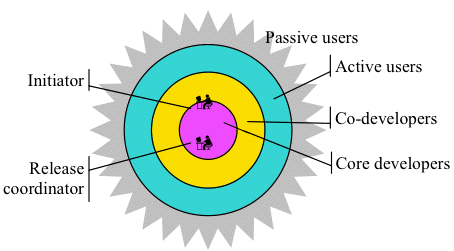
\includegraphics[width=0.6\textwidth]{figures/onion_model.png}
    \caption{Onion model of collaboration types in FLOSS projects \cite{crowstonSocialStructureFree2005}.}
    \label{fig:onion1}
\end{figure}

The onion model describes the types of participants in an OSS project as layers. The center represents the small group of core developers, who are responsible for the majority of contributions to the software. They are surrounded by a larger group of co-developers, whose main contributions are usually bug fixes reported by the active users. The passive users are usually the largest in numbers, who do not contribute or report any bugs. In a healthy FLOSS project, each layer of contributors are about one magnitude larger in numbers than the preceeding inner layer \cite{mockusTwoCaseStudies2002}. \\

% AUTHOR NAME HARDCODED HERE
El Asir et al. \cite{elasriPeripheryCoreTemporal2017} used a K-means classification to categorise project participants into a similar core-periphery structure (core, gray in-between area, and periphery) based on SNA metrics with a montly timeframe, and analysed how and why contributors transition between groups. They found that technical contributions like code commits and lines added have a much heavier impact on becoming a core developer as opposed to other activities, such as testing, reviewing and commenting. \\

% AUTHOR NAME HARDCODED HERE
A literature review conducted by McClean et al. \cite{mccleanSocialNetworkAnalysis2021} systematically analysed the state-of-the-art research of 46 scientific papers in the field of FLOSS social networks, and categorised them into three groups based on topic: structure, lifecycle and communication. They conclude, that the existence of core-periphery structure in OSS projects is well established in the field, which is also an indicator of a healthy FLOSS software. Regarding the lifecycle, generally the core development team does not change significantly over time, however, the project becomes more decentralised and distributed as it matures. A lack of research regarding temporal analyses were identified in the most current knowledge, which was suggested as a future research area in this field. \\

\subsection{Social network of Open-source projects}
In a larger FLOSS project, developers usually cannot understand every part of the project, therefore collaboration is required with eachother. The network created by the collaborators can be considered as a social network, because collaboration requires some kind of social interaction with eachother. Social network theory describes how social interaction patterns affect the individual behaviour \cite{martinez-torresGeneticSearchPatterns2012}. We can model an OSS project's social network as a graph, where nodes represent collaborators (developers, bug reporters, etc\dots) and edges represent the social interaction between them. In mathematical terms\dots \\

The type of the social interaction determines the created network, therefore choosing the basis of collaboration can have a significant impact on the network structure. The common types of developer social networks (DSNs) are Version Control System-based (VCS-DSN), Bug Tracking System-based (BTS-DSN) networks and DNSs, that are purely based on social elements \cite{aljemabiEmpiricalStudyEvolution2018}. The VCS-DSN take the version control application as a source for network generation by recording collaboration based on co-edits of the same module, file or code section. Choosing the granularity can impact the precision of true collaborations represented in the network. Co-edits by multiple developers to a single module or file does not necessarily mean actual collaboration was required from the authors, as the parts edited could work functionally independent from eachother. By increasing the granularity to file sections (classes or functions within a single file) or even lines, we can be more certain, that coordination was required, but we risk leaving out semantically connected parts of the project \cite{joblinEvolutionaryTrendsDeveloper2017}. In contrast to VCS-DSNs' purely technical approach, the BTS-DSNs use semi-technical bases for connecting participants, such as comments on issues, bugs or reviews \cite{elasriPeripheryCoreTemporal2017}. These artifacts, although being tightly related to specific sections of the source code, allow for taking into account conversational elements as contribution. For example, participants, who do not contribute directly to the software source code, but actively review and comment, are also considered. Lastly, social networks of developers can be constructed on project participation, following, starring or through communication means like mailing lists. The technical aspect of collaboration is minimized in such DNSs, and they are more fit for project organization and communication analyses in FLOSS projects (mailing list vs file file edits vs line edits) \\


% \subsubsection{Global SNA metrics}

% \subsubsection{Local SNA metrics}

%\begin{itemize}
%   \item Relevant social aspects of OS projects
%   \item State of the art
%   \item Collaboration by coediting files
%   \item Contributors form dynamic social networks
%    \item Problem of analysing changes over time in a network
%   \item Other studies in this field...
%\end{itemize}

\subsection{OSS project success}
community maturity (\cite{linBlogCommunityDiscovery2007} in \cite{aljemabiEmpiricalStudyEvolution2018}) \\

"Successful projects will likely have modular structure from the start or after refactoring as the source code grows larger and more unwieldy" \cite{antwerpEvolutionOpenSource2010} \\

success factors: Average Time Efforts, Number of Developers, Comments, Total Code Lines, Comment Ratio, Number of Rater \cite{yangHowMicrobloggingNetworks2013}
Truck Factor \cite{avelinoNovelApproachEstimating2016}


\section{Motivation of research problem and research questions}
Because there is a high dependency on the community in open source software projects, by understanding how contributions are included and what patterns emerge we can gain valuable insight into the project's current state and its trajectory. As stated before, SNA analysis of OSS have been extensively studied, but there is a lack of research regarding temporal models analyzing the lifecycle of a FLOSS project. \\

The goal of this paper is to fill in this gap by examining OSS project collaboration networks over time using SNA metrics. More specifically, one part of the research will focus on the evolution of such collaboration networks and comparing and contrasting these networks with the software outcome. The second part will focus on events during a project, and how it affects the developer collaboration. The research questions, which are broken down into subquestions, are as follows:

\begin{enumerate}
    \item \textbf{How does the temporal lifecycle information of a project influence its success?} \\
    
    \begin{enumerate}
        \item \textit{Based on temporal models of collaboration, is it possible to predict the outcome of the project?} Since it has been proven that the core collaborators do not change much over the course of the OS software development, our assumption is that any sudden or long-term change, that is not consistent with the other observed projects, can have a significant impact on the outcome (negative or positive alike).
        \item \textit{Can stages of a FLOSS project with a maturity model be observed?} As most OS software starts with a small collaborator basis and grows over time, it can be assumed, that each project goes through the same steps of open source maturity levels. On the other hand, it is also possible that due to the uniqueness of each project, no such stages are observable. 
    \end{enumerate}

    \item \textbf{How do major events in the project lifecycle change the collaboration network of the project?}
    \begin{enumerate}
        \item \textit{Do planned or foreseeable events change the collaboration structure?} Major software version releases can be considered foreseeable events of the project lifecycle, which could have an effect on the developer collaboration. For example, there might be a higher rate of interaction between contributors just before a new version is released to clear up the backlog of tasks. But it is also possible, that commit and change rates drop during this time, because the focus shifts to stability and testing instead of new features.
        \item \textit{How unforeseeable internal or external events affect FLOSS collaboration?} Sudden shocks to the project, such as an announcement of disinterest from major users of the software, discontinued enterprise support of the project, large-scale global events like the pandemic, or sudden employee firings can have significant effect on the core and periphery collaborators alike. By analysing the collaboration network before, during and after such changes, we might be able to recognise patterns, that regularly occur around these events.
    \end{enumerate}
\end{enumerate}

\subsection{Research methodology}
To find answers to the research questions above, first we build a repository analyzer tool, which mines collaboration data from FLOSS projects, generates static snapshot collaboration networks at each given time interval and calculates SNA metrics for each snapshot. Then these metrics can be aggregated over time, or plotted against time to discover changes in the network. The \texttt{git2net}\footnote{\url{https://github.com/gotec/git2net}} \cite{goteAnalysingTimeStampedCoEditing2019} Python library provides the necessary tools to mine any project repository that uses git version control. It also incorporates temporal network generation capability, which can be used as a source for creating static collaboration networks aggregated over a given period of time. \\


We apply a hybrid methodology of qualitative and quantitative research. First, as part of the qualitative research, we choose a small number of repositories to be analyzed. We observe the number of connected components, centrality, number of nodes and mean degree SNA metrics in order to discover the core and peripherial collaborators over the project lifecycles. The basis of collaboration, due to the unavailability of other means of communication, is coediting files. Based on the state of the art research in this field, file coediting proves to be an effective and easy way to represent collaboration between developers. \\

After discovering the collaboration structure over time, we will match the breakpoints and unexpected spikes or troughs to events within the lifespan of the project. We expect that the key SNA metrics will show a periodicity around planned releases and other reoccurring events (e.g. holiday season). Outstanding values without reoccurrence, on the other hand, are more likely to be consequences of unexpected events. In these cases, it should be observed whether the network is capable of reorganizing itself, or does the event leave a permanent mark on the collaboration structure. A categorization of unexpected events and the level of impact each category has should be observed. \\

For the quantitative research to be conducted, we will gather a large set of repositories along with major events in its lifecycles. We will then run the miner for all repositories, and with the findings of the qualitative research, we will try to detect all major events and their type (planned or unexpected). We will utilize the \texttt{ruptures} \footnote{\url{https://github.com/deepcharles/ruptures}} library to detect changes in the continuous SNA metrics. If the model is capable to accurately recognise events, then we can also apply it on any repository to detect changes, which will allow us to discover changes in the collaboration network that are not related to publicly known events or releases. \\

% Quantitative research
% \begin{itemize}
%     \item Composing a large set of repositories (different sizes, properties) with their success or failure
%     \item Gathering major events for the repositories (version releases, external events, global events)
%     \item Detecting past changes automatically based on changes in measured statistics
%     \item How do changes and reoccurring patterns match the events?
%     \item What structures can be noticed before a major success or failure of a project?
% \end{itemize}


\section{Gitminer implementation}
To find answers to the research questions, we implement an analysis tool to mine and analyze project repositories, which allows us to generate collaboration networks and network metrics for the analysed projects. \\

\subsection{\texttt{git2net} miner}
The process begins with the project mining. After cloning the repository, the \texttt{git2net} \cite{goteAnalysingTimeStampedCoEditing2019} library is used to collect data related to commits. Specifically, who is the author of each commit, which files were modified (created, edited, deleted) with the commit, and when was the commit created. Additionally, the lines edited by the author within each commit are collected separately, allowing for a more fine-grained collaboration network generation if necessary. The results are collected into an \texttt{sqlite} \footnote{\url{https://www.sqlite.org/index.html}} database file's \textit{commits} and \textit{edits} tables. \\

The \texttt{git2net} mining process by default collects all the commits throughout the project's lifecycle. However, the processing time of each commit differs based on the number of edits, the affected number of files and the file types as well, which makes collecting certain commits very resource-intense and time-costly. Therefore, we exclude every commit, which contains more than 100 file modifications, during each repository mining using the \textit{max\_modifications} parameter. As observed by Gote et al \cite{goteAnalysingTimeStampedCoEditing2019}, this exclusion criteria does not affect significanly the generated network, because they are mostly merge commits or project restructurings, which do not mark any true collaboration effort between developers. During the data mining in certain repositories, we encountered commits, that were not mineable with this method and the mining process halted, presumably due to processing error because of binary file changes in these commits. We also excluded these commits from our data mining process.\\

This exclusion criteria resulted in an average of 3\% of commits excluded in all repositories subject to our analyses, with the highest excluded commit rate being 20\%.

\subsection{\texttt{repo\_tools} miner} 

We use the \texttt{repo\_tools} \footnote{\url{https://github.com/wschuell/repo\_tools/}} Python library to query the Github API for additional repository data extraction, such as:

\begin{itemize}
    \item Releases
    \item Tags
    \item Issues
    \item Stars and followers
\end{itemize}

The mining output is also stored in a \texttt{sqlite} relational database, which is queried later on during the analysis. 

% - what do we want to achieve with the gitminer
%  - generate networks of collaboration
%    - what should be the basis of collaboration
%  - filter for time
%  - generate statistics

\subsection{Data preprocessing}

The collaboration networks with the \texttt{git2net} library connect the authors to their edited files using only file and author names instead of IDs. This creates an issue when generating the networks, because authors with the same name will show up as one node, and they will be connected to the files they touched combined. Furthermore, authors that change their displayed name ('author\_name' field in the mining database) or log in from diferent accounts, where they have different names, will show up as multiple nodes instead of a single vertex. \\

We utilize the \texttt{gambit} \cite{goteGambitOpenSource2021} rule-based disambiguation tool to resolve the author names. Furthermore, the created networks have issues when the node names contain special characters or spaces. Therefore, after disambiguation, we replace every unique author name with its ID number. \\

As the files are also labelled by their filename property in the network outputs, the same filenames but in different folders are also displayed as single nodes. In order not to create false collaborations, we simply remove the files from the network with filenames, that occur more than once in all the repository subdirectories. We argue that this does not remove any significant collaboration data, since most files sharing their name with other files are technicaly files, like \texttt{\_\_init\_\_.py} for a Python project. \\

\subsection{Collaboration networks}

When creating a DSN from the mined data, we have multiple methods at hand. The \texttt{git2net} library provides its own co-editing network function, which returns a temporal network of collaborators. This uses the co-authorship algorithm developed by Gote et. al. \cite{goteAnalysingTimeStampedCoEditing2019}, however, we would like to have more control over the network generation method, such as simple file-based co-authorship in order to customize the network for our needs, like weighing each relation or generating undirected graphs. \\

\subsubsection{Temporal bipartite network}
As a first step, we generate a temporal bipartite network of authors and their edited files with the \texttt{git2net} built-in \textit{get\_bipartite\_network} method. A temporal network is a \texttt{pathpy} \footnote{\url{https://www.pathpy.net/}} graph object, which contains a collection of timestamped graphs of a single network at each point in time within the observed timeframe. Such a snapshot $S_t = (U, V, E_t)$, where $U$ is the set of authors, $V$ is the set of files and $E_t$ is the set of file edits as edges at $t$ timestamp. By connecting the authors, who touched the same files, and removing the nodes representing the edited files (converting the bipartite network to a regular network), we can observe the evolution of the collaboration over time, represented in Figure \ref{fig:temporal net}. \\

\begin{figure}
    \centering
    \begin{subfigure}{0.3\textwidth}
        \centering
        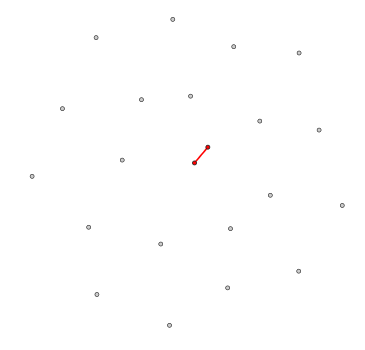
\includegraphics[width=0.92\textwidth]{figures/temporal/0.png}
        \caption{}
        \label{fig:temporal net A}
    \end{subfigure}
    \hfill
    \begin{subfigure}{0.3\textwidth}
        \centering
        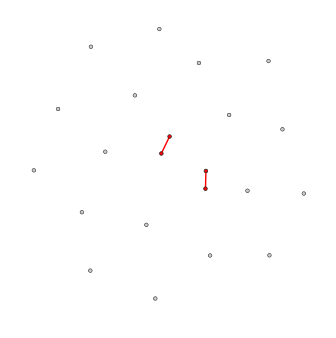
\includegraphics[width=0.92\textwidth]{figures/temporal/1.png}
        \caption{}
        \label{fig:temporal net B}
    \end{subfigure}
    \hfill
    \begin{subfigure}{0.3\textwidth}
        \centering
        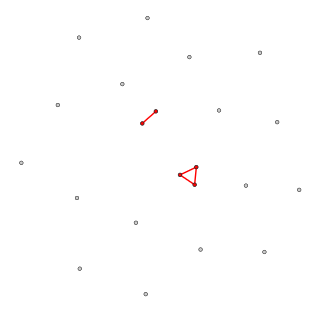
\includegraphics[width=0.92\textwidth]{figures/temporal/2.png}
        \caption{}
        \label{fig:temporal net C}
    \end{subfigure}
    \hfill
    \begin{subfigure}{0.3\textwidth}
        \centering
        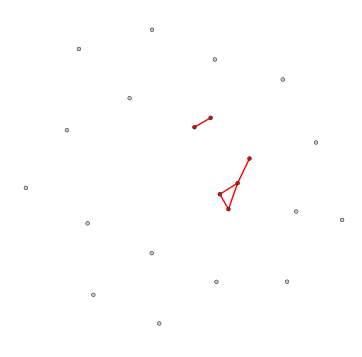
\includegraphics[width=0.92\textwidth]{figures/temporal/3.png}
        \caption{}
        \label{fig:temporal net D}
    \end{subfigure}
    \hfill
    \begin{subfigure}{0.3\textwidth}
        \centering
        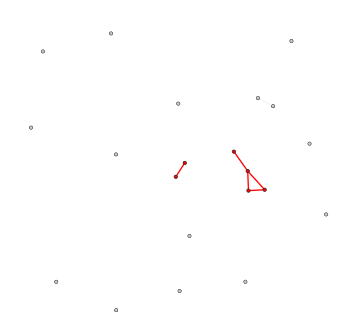
\includegraphics[width=0.92\textwidth]{figures/temporal/4.png}
        \caption{}
        \label{fig:temporal net E}
    \end{subfigure}
    \hfill
    \begin{subfigure}{0.3\textwidth}
        \centering
        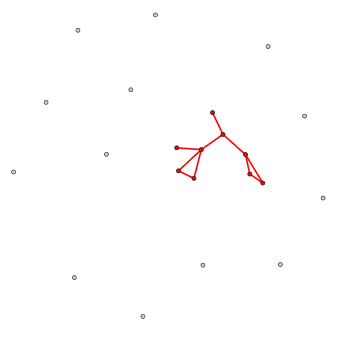
\includegraphics[width=0.92\textwidth]{figures/temporal/5.png}
        \caption{}
        \label{fig:temporal net F}
    \end{subfigure}
    \caption{Sequential snapshots of the \texttt{networkx} collaboration network with a moving time-window of 30 days and 7-day steps.}
    \label{fig:temporal net}
\end{figure}

Although a temporal network preserves the time aspect of the graph by the edges being tied to the time dimension of the graph, calculating network metrics like centrality on such networks is infeasible. Visualization also proves to be difficult in representations where animation is not possible. Therefore, we aggregate the bipartite network over a given timeframe into a static network. All nodes within the temporal net are preserved, and all directed edges are added to the network with the edge weight representing how many times that author edited the file. \\

\subsubsection{Static networks}
The generated static weighed bipartite network looses its time-varying component, but now we are able to manipulate and calculate complex statistics over it. Figure \ref{fig:bipartite} is an example of such a network. As a next step, we convert the the bipartite network into an authors' network by removing the nodes representing files. \\

\begin{figure}
    \centering
    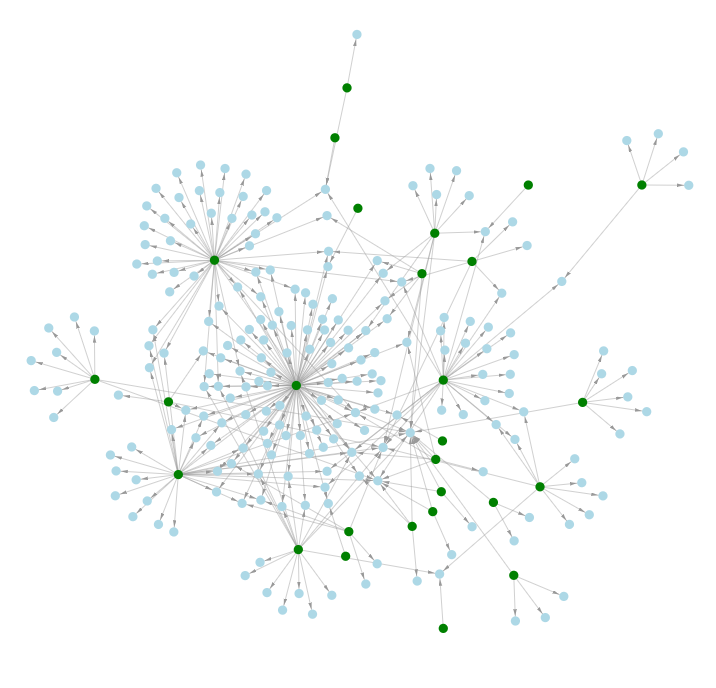
\includegraphics[width=0.65\textwidth]{figures/bipartite.png}
    \caption{A bipartite network of authors (green) and edited files (light blue) in the \texttt{pandas} project within the timeframe 31/01/2021 and 15/02/2021}
    \label{fig:bipartite}
\end{figure}

We have multiple methods to convert the directed and weighted bipartite network into a projection of authors. We could simply remove the files and connect each author, that worked on the same file, however, the end result would be an unweighted graph. This would falsely show, that all collaborations are weighed equally, which is clearly not the case, as multiple continuous edits on the same file from both parties should represent a stronger collaborative connection. Therefore, firstly we implement the Weighted One-Mode Projection (WOMP) method \cite{stramWeightedOneMode2017}, The WOMP method converts the bipartite network $G(A,F,E)$, where $E$ is the edge list containing tuples $(a_i,f_i,w_{ij})$, and $w_{ij} \in E$ is the weight between author $a_i \in A$ and file $f_i \in F$. With this notation, a weighted directed edge can be calculated for any $a_a, a_b \in A$ as follows:

\[ w_{ab}^{A \rightarrow A} = \sum_{j=1}^m \frac{w_{aj}}{W_a^F}, \]

where $W_a^F$ is the sum of all outgoing edge weights from author $a$ to all files $F$ denoted as $W_a^F = \sum_{i=1}^n w_{ai}$. This creates a bidirectional weighted collaboration network between authors $a_1$ and $a_2$, where the weight $w_{12}$ represents the relative collaboration effort of $a_1$ towards $a_2$ compared to all the other developers $a_1$ has collaborated with. Conseqently, every edge is in the rage $[0,1]$ in the resulting WOMP network. \\

A disadvantage of the WOMP method is, that the generated collaboration network is bidirectional, meaning if there was any common authored files between $a_1$ and $a_2$, then there will be both $w_{12}$ and $w_{21}$ connecting them. To simplify the network, we want to generate an authors network, where the edges are undirected. For this, we are using the weighted Jaccard method on the files-authors bipartite network:

\[ w_{ab} = \frac{\sum_{f \in F}min(f_a, f_b)}{\sum_{f \in F}max(f_a, f_b)}. \]

For each file $f$ that $a_1$ and $a_2$ authors touch, we sum up the minimum and maximum weights the authors have towards each file, then we divide the sum of minimums with the sum of maximums. This results in the undirected author-author network with edge weights in range $[0, 1]$. By default, this method removes isolated contributors, who do not collaborate with eachother, but are actively editing the files. We add these nodes manually. Figure \ref{fig:jaccard} shows the final author network. \\

\begin{figure}
    \centering
    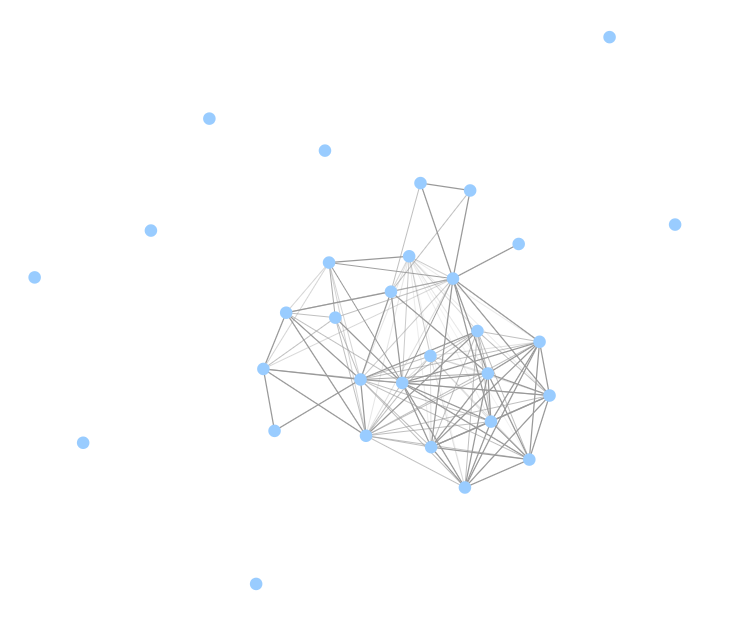
\includegraphics[width=0.9\textwidth]{figures/jaccard.png}
    \caption{Weighted Jaccard similarity collaboration network of \texttt{pandas} generated from the bipartite network in Figure \ref{fig:bipartite}.}
    \label{fig:jaccard}
\end{figure}

\subsection{Core and periphery, centralization}
A critical part of the OSS software projects is the existence of core and periphery developers. It has been observed, that in each FLOSS project there are a small number of developers, who provide the vast majority of development effort into the project. It has been also established, that the members of core developers do not change substantially during the project's lifecycle. However, there was no effort on whether there is a change in the collaboration pattern, especially before, during or after a major lifecycle event. Therefore, we make efforts identifying the core developer network to observe these changes. \\

\subsubsection{Degree centrality}

We use the degree centrality of each node (i.e. developer) to identify the core members. Degree centrality of a node is the fraction of all possible nodes it is connected to. We can calculate it by dividing the degree with $n-1$, where $n = |G|$ the number of nodes within the network. Since the core developers contribute the majority of commits and edits of the project, they are expected to be connected with more nodes. Joblin et. al. \cite{joblinClassifyingDevelopersCore2016, joblinEvolutionaryTrendsDeveloper2017} have also identified degree centrality as the best predictor of core developers. In cases, where binary classification of core or periphery is needed, we assign developers to the core network if their degree centrality score is in the top 20th percentile, otherwise they are considered as periphery. We also take note, that this method does not consider the weighted edges, only the number of edges (degree) a node has. Although this method could be refined to consider the node degree weighted with the edges, we argue that this could lead to invalidity. In case of two developers, who only contributed to one file, they will be represented with a strong connection and would receive a high weighted degree value, whereas a core contributor, who edits many files, can have many weak connections but these might not add up to one strong connection of the two isolated developers when weighted with the edge weights. It is clear, that a developer with many connections, regardless of the strength of the collaboration, should be considered core. \\

\begin{figure}
    \centering
    \begin{subfigure}{0.49\textwidth}
        \centering
        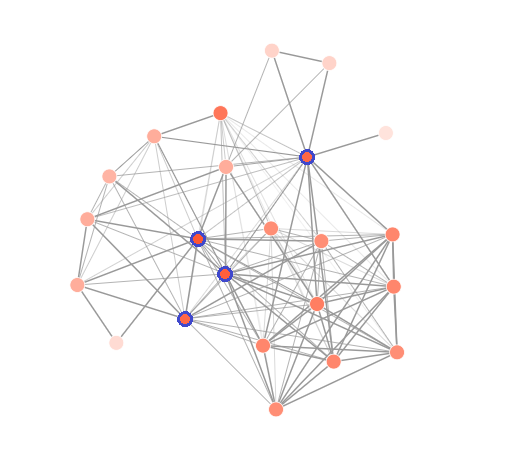
\includegraphics[width=0.98\textwidth]{figures/degree_centrality.png}
        \caption{Pandas}
        \label{fig:centrality a}
    \end{subfigure}
    \hfill
    \begin{subfigure}{0.49\textwidth}
        \centering
        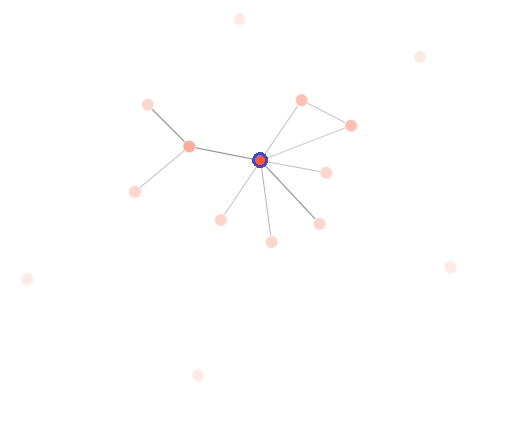
\includegraphics[width=0.98\textwidth]{figures/degree_centrality_curl.png}
        \caption{Curl}
        \label{fig:centrality b}
    \end{subfigure}
    \caption{Degree centrality within the \texttt{pandas} and \texttt{curl} projects' collaboration networks. Darker colors represent a higher degree centrality value. The  highlighted nodes are in the highest 20th percentile of degree centrality, classifying as members of the core developers. We can observe in both one-month periods, that \texttt{pandas} is much more decentralized, whereas \texttt{curl} is largely dependent on one developer.}
    \label{fig:degree centrality}
\end{figure}

\subsubsection{Degree centralization}

The degree \textit{centrality} can be calculated for every node, however, through our analysis we would also like to measue a global \textit{centralization} metric, which is applicable to the whole network. As suggested by Crowston and Howison \cite{crowstonHierarchyCentralizationFree2006}, we calculate the degree \textit{centralization} by summing the differences between the maximum and each node's degree \textit{centrality}. 

\[ C_D(A) = \frac{\sum_{i=1}^n(C_d(a*)-C_d(a_i))}{H}, \]

where $C_d(a)$ is the degree \textit{centrality} of an author $a$, $a*$ is the author with the highest degree \textit{centrality} value, and $n$ is the number of authors in the collaboration network $A$. The value $H$ is for normalizing the sum by dividing by the theoretical maximum \textit{centralization}. Since the \textit{centrality} values are already in the range $[0, 1]$, we only need to normalize for the network's size. We get the highest centrality score with a star graph, where each node is only connected to a single central node, which has exactly one edge to all other nodes. The central node has a centrality of 1 in this case, whereas all the other $n-1$ nodes have $C_d(a) = \frac{1}{n-1}$. This means that in case of a star graph:

\[ H = (n-1) (1-\frac{1}{n-1}) = n-2. \]

Within certain timeframes, when a project is inactive, it could happen, that the network contains 2 nodes or less. We define $C_D(A) = 0$ if $|A| = n <=2$. The resulting output will always have a value in $[0, 1]$, where 1 means a completely centralized network (star graph) and 0 means a completely decentralized network. It is important to emphasize that a centralization score of 0 does not necessarily mean that there is no collaboration and every developer is isolated. Rather it means that each developer is co-authoring with just as many authors, as the others do. \\

% - Gini coefficient

% - \cite{klugUnderstandingGroupDynamics}

\subsubsection{Clustering coefficient}

While centralization helps us describe the centralness of the network and how much it is centered around a single, or a small number of developers, it does not help us describing the structure of the network in more detail. Our goal is to gain an understanding of also the modularity of our network, meaning how much developers tend to cluster together \cite{joblinEvolutionaryTrendsDeveloper2017}. We expect that authors form smaller clusters, which are more tightly connected together, and these clusters have somewhat weaker ties to other clusters. This builds on the assumption that the social network of the software follows the modules which build up the software itself, thus authors of a specific function should also cluster together within the network \cite{conwayHowCommitteesInvent1968, joblinEvolutionaryTrendsDeveloper2017}. To measure this "clusteredness", we calculate the \textit{local clustering coefficient} for each node. \\

\begin{figure}
    \centering
    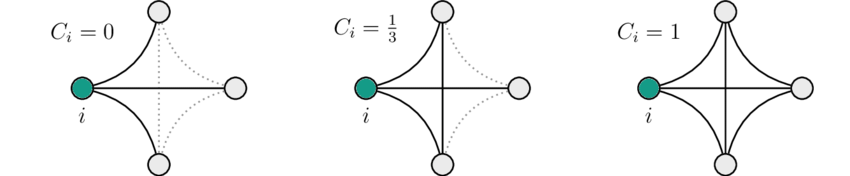
\includegraphics[width=1\textwidth]{figures/loc_clust_coeff.png}
    \caption{The local clustering coefficient demonstrated on an unweighted network of 4 vertices \cite{jedrzejewskiRoleComplexNetworks2016}.}
    \label{fig:loc clust coeff}
\end{figure}

The \textit{local clustering coefficient} quantifies on a scale $[0, 1]$ how likely it is that a node's neighbours are also neighbours. We use the number of how many triangles (also called clique, triplet) is every node a part of. This is illustrated for unweighted networks on Figure \ref{fig:loc clust coeff} with the formula:

\[ C_i = \frac{2T(i)}{deg(i)(deg(i)-1)}, \]

where $T(i)$ is the number of triangles through node $i$ and $deg(i)$ is the degree of i. However, in a weighted network we also have to consider the edge weights, since it is easy to see that a clustering coefficient of 1 with also the maximum weighted edges in a triplet does not represent the same clustering as being connected with a weak links. We expect weaker links connecting larger clusters, whereas stronger links within each cluster. Therefore, we use geometric averaging of the subgraph edge weights (as implemented by the \texttt{networkx}\footnote{\url{https://networkx.org/documentation/stable/reference/algorithms/generated/networkx.algorithms.cluster.clustering.html}} library \cite{onnelaIntensityCoherenceMotifs2005}):

\[ c_i = \frac{\sum_{jk}(\hat{w}_{ij}\hat{w}_{ik}\hat{w}_{jk})^{1/3}}{deg(i)(deg(i)-1)}. \]

The $\hat{w}_{ij}$ represents the normalized weight of edge $e_{ij}$ over the maximum weight in the network. \\

\subsubsection{Hierarchy}
The degree centrality and the clustering coefficient are in themselves able to express meaningful aspects of the developer social network, however, by combining the two metrics, we can also assess how hierarchical the network is. In a scale-free social hierarchical network (such as the collaboration network), nodes tend to cluster around a single or a few hubs, which are more likely to have weak connections to other hubs \cite{ravaszHierarchicalOrganizationComplex2003, joblinEvolutionaryTrendsDeveloper2017}. The nodes within these formed groups are relatively stronger than the connections connecting the hubs, but they are less likely to connect to nodes outside of their group. Therefore in a hierarchical network, the hubs have a high degree number and a low clustering coefficient, whereas the group members clustering around the hubs have a high clustering coefficient, but low degree numbers. \\

We can visualize the degree of hierarchy by plotting each node's  clustering coefficient against the number of degrees, shown in Figure \ref{fig:hierarchy}. In hierarchical networks, the plotted linear regression trendline will decrease steeply, as there is a negative correlation between the degree and clustering coefficient. In networks, where this cannot be observed, the trendline stays flat, meaning these two metrics are independent from eachother and the structure is not hierarchical. To measure the hierarchical level numerically within a network, we take the trendline's slope, which is $\beta_1$ in the $y=\beta_1x + \beta_0$ general linear regression equation. \\

\begin{figure}
    \centering
    \begin{subfigure}{0.49\textwidth}
        \centering
        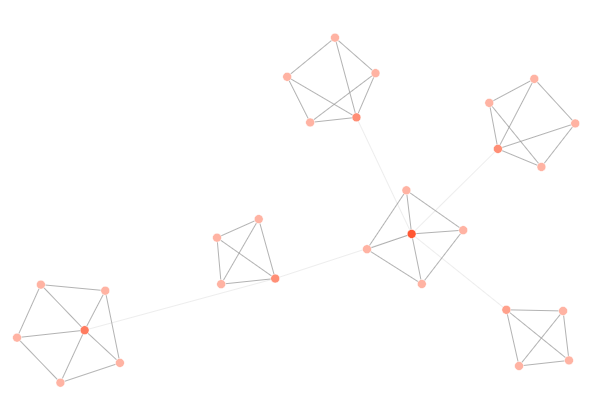
\includegraphics[width=0.98\textwidth]{figures/hierarchical.png}
        \caption{Highly hierarchical network}
        \label{fig:hierarchical}
    \end{subfigure}
    \hfill
    \begin{subfigure}{0.49\textwidth}
        \centering
        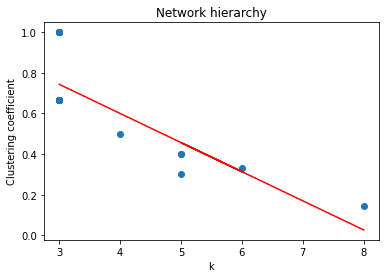
\includegraphics[width=0.98\textwidth]{figures/hierarchy_plot.png}
        \caption{Network hierarchy}
        \label{fig:hierarchy plot}
    \end{subfigure}
    \caption{Hierarchical network and its corresponding degree number vs clustering coefficient plot.}
    \label{fig:hierarchy}
\end{figure}

In every network isolated authors can be observed, who are only working on files that noone else has edited (in the given timeframe). These nodes can skew the hierarchy score, because an isolated node's degree and clustering coefficient are by definition 0, which disproportionately makes the trendline much flatter. Therefore, we remove the isolated nodes from the network. If the network only contains isolated nodes, and there is no linear regression to be calculated, we set the hierarchy value to 0.

\subsubsection{Release measures}
% - issues opened
% - issues closed
% - avg issue open time
% - more... from: \cite{jarczykSurgicalTeamsGitHub2018}

\subsection{Time window}
% - Time window scanning over time
% - parameters: delta, interval, from, to
% - size of the project matters
% - activity determines the scale (less activity = small interval (week), vice versa)
% - helps: commits per day plot (insert)

% - The efficiency of a project’s workflow (measured by the percentagesof issues assigned to specific developers). \cite{jarczykSurgicalTeamsGitHub2018}




\section{Collaboration pattern analysis}
\subsection{Observed projects and events}
% - which projects (Servo, pandas, numpy, networkx, seaborn, wasmtime, ruptures (?))
% - expected: Big releases
% - unexpected: layoffs
\subsection{SNA metrics analysis}
\subsubsection{K-cores}
Besides taking the 20th percentile of the top clustering coefficients to identify the number of core developers in the network, we ....
% - 20th percentile of k-core nodes
% - alternative to identifying the core members
%....
\subsection{Results}
%....


% (\item Automatic event recognition)
%     (\item Event detection implementation (ruptures))
%     (\item Collaboration network change detection)
\section{Quantitative analysis of projects during crunch time}
\subsection{Collaboration network changes}
\subsection{Prediction of outcome based on collaboration changes}

\section{Discussion and results}
\section{Conclusion and future work}


\Urlmuskip=0mu plus 1mu\relax
\bibliographystyle{plain}
%\bibliographystyle{plainnat}
\bibliography{References}

\newpage

\let\svaddcontentsline\addcontentsline
\renewcommand\addcontentsline[3]{%
  \ifthenelse{\equal{#1}{lof}}{}%
  {\ifthenelse{\equal{#1}{lot}}{}{\svaddcontentsline{#1}{#2}{#3}}}}
\begin{appendices}
    \section{Connected components over time}
    \begin{figure}[h!]
       \centering
       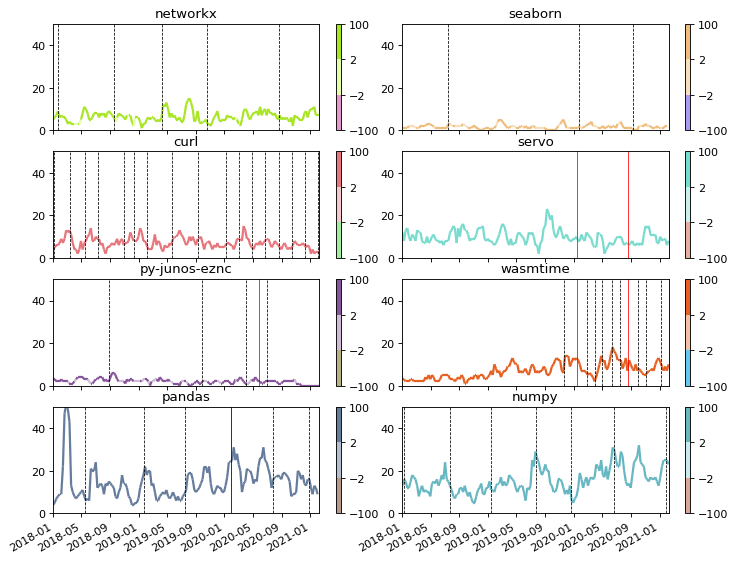
\includegraphics[width=\textwidth]{figures/qualitative/connected components/components.png}
       \caption{Connected components}
       \label{fig:components}
    \end{figure}

    \section{Randomized repository selection}
    \label{app:repos}
    \begin{center}
        %\resizebox{\textwidth}{!}{%
        %\footnotesize%%%%%%%%%%%  smaller font size %%%%%%%%
        \begin{longtable}{|l|l|l|}
            \caption{Randomized selection of repositories.}\\
            \hline
            \textbf{Mining} & \textbf{Name} & \textbf{Created at} \\
            \hline
            \endfirsthead
            \multicolumn{3}{c}%
            {\tablename\ \thetable\ -- \textit{Continued from previous page}} \\
            \hline
            \textbf{Mining} & \textbf{Name} & \textbf{Created at} \\
            \hline
            \endhead
            \hline \multicolumn{3}{r}{\textit{Continued on next page}} \\
            \endfoot
            \hline
            \endlastfoot
            OK & ansible/awx & 17/5/2017 15:50 \\
            mining err & antennapod/antennapod & 31/7/2012 10:25 \\
            bad ver & apache/lucenenet & 27/3/2009 15:41 \\
            OK & apinf/platform & 4/3/2015 8:33 \\
            OK & aria2/aria2 & 27/11/2010 9:41 \\
            bad ver & arvidn/libtorrent & 3/6/2015 5:22 \\
            OK & astropy/halotools & 9/1/2015 21:43 \\
            mining err & augurproject/augur-ui & 2/2/2015 20:56 \\
            bad ver & azure/azure-sdk-for-net & 6/12/2011 23:32 \\
            OK & betaflight/betaflight-configurator & 8/6/2016 22:32 \\
            OK & bitzenycoredevelopers/bitzeny & 24/10/2017 14:48 \\
            OK & boost-ext/di & 23/1/2012 21:42 \\
            OK & canjs/canjs & 20/1/2012 17:57 \\
            bad ver & cegui/cegui & 9/1/2020 8:15 \\
            bad ver & chakra-ui/chakra-ui & 17/8/2019 14:27 \\
            bad ver & clasp-developers/clasp & 20/5/2014 3:54 \\
            mining err & corretto/corretto-11 & 11/2/2019 20:13 \\
            OK & dbeaver/dbeaver & 21/10/2015 8:26 \\
            OK & dgcdev/digitalcoin & 8/9/2014 9:58 \\
            OK & dhis2/dhis2-android-capture-app & 11/4/2018 17:1 \\
            OK & digitalgreenorg/dg & 9/11/2011 16:4 \\
            bad ver & dimagi/commcare-hq & 9/7/2009 17:0 \\
            OK & dita-ot/dita-ot & 14/4/2012 4:49 \\
            OK & ember-cli/ember-cli & 3/11/2013 17:34 \\
            OK & endless-sky/endless-sky & 14/3/2015 20:44 \\
            mining err & euroelessar/qutim & 18/5/2011 14:56 \\
            OK & fioprotocol/fio & 3/3/2020 20:2 \\
            bad ver & firemodels/smv & 31/8/2016 15:46 \\
            OK & flowminder/flowkit & 31/10/2018 23:59 \\
            bad ver & foam-framework/foam & 1/5/2014 18:10 \\
            mining err & frappe/erpnext & 8/6/2011 8:20 \\
            OK & geli-lms/geli & 14/3/2017 13:56 \\
            bad ver & gemini-hlsw/ocs & 12/9/2014 14:20 \\
            OK & geonetwork/core-geonetwork & 14/6/2012 9:59 \\
            OK & globalarrays/ga & 17/2/2017 20:48 \\
            OK & gmod/jbrowse & 16/1/2009 11:30 \\
            bad ver & gulden/gulden-official & 13/8/2015 10:46 \\
            mining err & handsontable/handsontable & 23/5/2011 22:38 \\
            OK & ibm/carbon-components-angular & 31/7/2018 19:41 \\
            OK & imageengine/cortex & 12/6/2013 23:12 \\
            bad ver & intermine/intermine & 2/7/2012 10:25 \\
            bad ver & iotaledger/trinity-wallet & 23/5/2018 15:8 \\
            mining err & iov-one/iov-core & 17/4/2018 18:46 \\
            OK & jhipster/generator-jhipster & 21/10/2013 20:7 \\
            OK & kiwix/kiwix-android & 18/1/2017 19:48 \\
            OK & ksp-ro/realismoverhaul & 5/1/2014 23:2 \\
            OK & lavaio/lava & 3/6/2019 2:20 \\
            OK & ledgerhq/ledger-live-desktop & 21/2/2017 12:52 \\
            OK & linq2db/linq2db & 18/6/2011 16:24 \\
            OK & linuxdeepin/dde-control-center & 6/11/2013 7:23 \\
            mining err & liqd/adhocracy3 & 15/8/2014 8:7 \\
            mining err & liveblog/liveblog & 18/2/2015 9:22 \\
            mining err & livelykernel/livelykernel & 10/2/2012 0:31 \\
            bad ver & lk8000/lk8000 & 9/1/2011 16:55 \\
            OK & mavlink/qgroundcontrol & 13/10/2011 7:31 \\
            OK & megaglest/megaglest-source & 25/11/2013 21:10 \\
            bad ver & micro-ros/nuttx & 15/1/2018 14:29 \\
            bad ver & microsoft/azure-pipelines-tasks & 6/12/2014 11:11 \\
            mining err & microsoft/cntk & 26/11/2015 9:52 \\
            bad ver & microsoft/recommenders & 19/9/2018 10:6 \\
            bad ver & mozilla/addons-frontend & 19/2/2016 17:25 \\
            bad ver & mvvmcross/mvvmcross & 28/11/2011 22:45 \\
            OK & myhush/hush & 16/6/2017 14:37 \\
            OK & nccgroup/scoutsuite & 30/10/2018 11:46 \\
            bad ver & nfs-ganesha/nfs-ganesha & 2/11/2012 17:25 \\
            bad ver & nightscoutfoundation/xdrip & 23/9/2016 13:33 \\
            bad ver & nuget/nugetgallery & 9/8/2011 17:57 \\
            OK & nukeykt/nblood & 12/2/2019 13:57 \\
            OK & nunit/nunit & 18/10/2013 23:43 \\
            OK & open62541/open62541 & 20/12/2013 8:45 \\
            OK & openbazaar/openbazaar-desktop & 21/6/2016 14:34 \\
            OK & openzfs/zfs & 14/12/2009 20:20 \\
            mining err & pculture/miro & 31/8/2011 15:58 \\
            mining err & photonstorm/phaser & 12/4/2013 12:27 \\
            OK & pmeal/openpnm & 25/7/2013 20:32 \\
            OK & project-osrm/osrm-backend & 22/9/2011 10:5 \\
            OK & ptmt/react-native-macos & 4/10/2015 15:22 \\
            OK & real-logic/aeron & 7/2/2014 17:16 \\
            OK & reportportal/service-ui & 14/9/2016 12:38 \\
            OK & restcomm/sip-servlets & 17/8/2012 14:7 \\
            OK & rptools/maptool & 21/10/2014 12:26 \\
            OK & scipp/scipp & 6/9/2018 7:1 \\
            OK & secdev/scapy & 1/10/2015 17:6 \\
            OK & sefaria/sefaria-project & 20/9/2011 20:23 \\
            OK & simpeg/simpeg & 26/11/2013 19:46 \\
            OK & souffle-lang/souffle & 12/3/2016 3:39 \\
            OK & spongepowered/sponge & 11/4/2015 20:38 \\
            mining err & spongepowered/spongecommon & 11/4/2015 20:38 \\
            OK & spotbugs/spotbugs & 4/11/2016 22:18 \\
            OK & spyder-ide/spyder & 16/2/2015 22:49 \\
            OK & stack-of-tasks/pinocchio & 7/10/2014 15:42 \\
            OK & swaywm/sway & 5/8/2015 1:31 \\
            bad ver & syndesisio/syndesis & 2/10/2017 17:26 \\
            OK & taskcluster/taskcluster & 15/12/2018 3:48 \\
            OK & telefonicaid/fiware-orion & 13/9/2013 11:55 \\
            mining err & theano/theano & 10/8/2011 3:48 \\
            OK & tropy/tropy & 3/11/2015 21:29 \\
            OK & tryghost/ghost & 4/5/2013 11:9 \\
            OK & twbs/bootstrap & 29/7/2011 21:19 \\
            bad ver & ultimaker/cura & 16/6/2014 12:55 \\
            OK & unidata/netcdf-c & 6/8/2013 20:48 \\
            OK & unvanquished/unvanquished & 30/9/2011 16:44 \\
            bad ver & uportal-project/uportal & 20/10/2011 15:34 \\
            OK & visit-dav/visit & 13/1/2019 23:27 \\
            OK & vuetifyjs/vuetify & 12/9/2016 0:39 \\
            OK & wazuh/wazuh-kibana-app & 29/6/2016 1:43 \\
            mining err & zeebe-io/zeebe & 20/3/2016 3:38 \\
            bad ver & zenorogue/hyperrogue & 8/8/2015 13:53 \\
            OK & zephyrproject-rtos/zephyr & 26/5/2016 17:54 \\
            OK & zilliqa/zilliqa & 27/12/2017 7:42 \\
            \end{longtable}
        %}
        %\normalsize
    \end{center}
    
    \newpage

    \section{Boxplots}
    \label{app:boxplots}

    \begin{figure}[!htb]
        \centering
        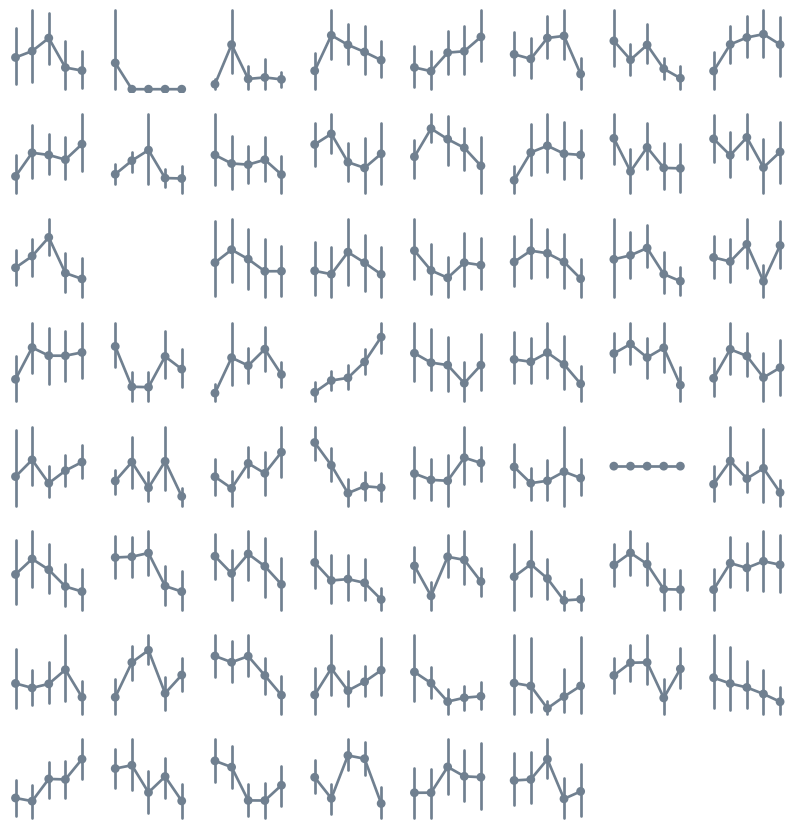
\includegraphics[width=\textwidth]{figures/quantitative/pointplots/mean_path_length_all.png}
        \caption{Boxplots for mean path length in all repositories mined.}
        \label{app:mean_path-box-app}
    \end{figure}

    \begin{figure}[!htb]
        \centering
        
\includegraphics[width=\textwidth]{figures/quantitative/pointplots/issues_opened_all.png}
        \caption{Boxplots for number of issues opened in all repositories mined.}
        \label{app:issues_opened-box-app}
    \end{figure}

    \begin{figure}[!htb]
        \centering
        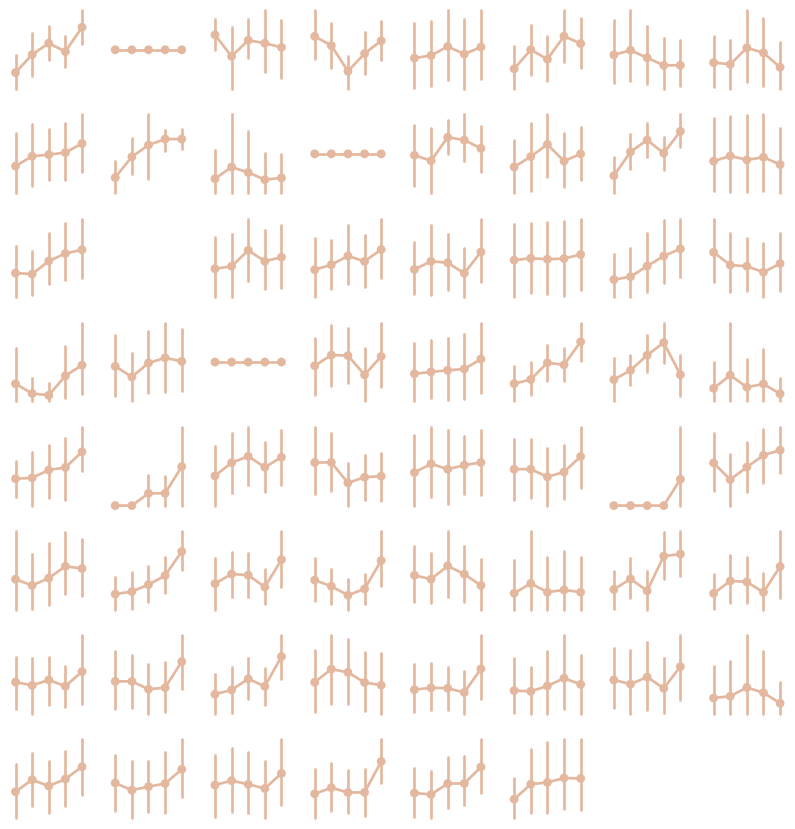
\includegraphics[width=\textwidth]{figures/quantitative/pointplots/issues_closed_all.png}
        \caption{Boxplots for number of issues closed  in all repositories mined.}
        \label{app:issues_closed-box-app}
    \end{figure}

    \begin{figure}[!htb]
        \centering
        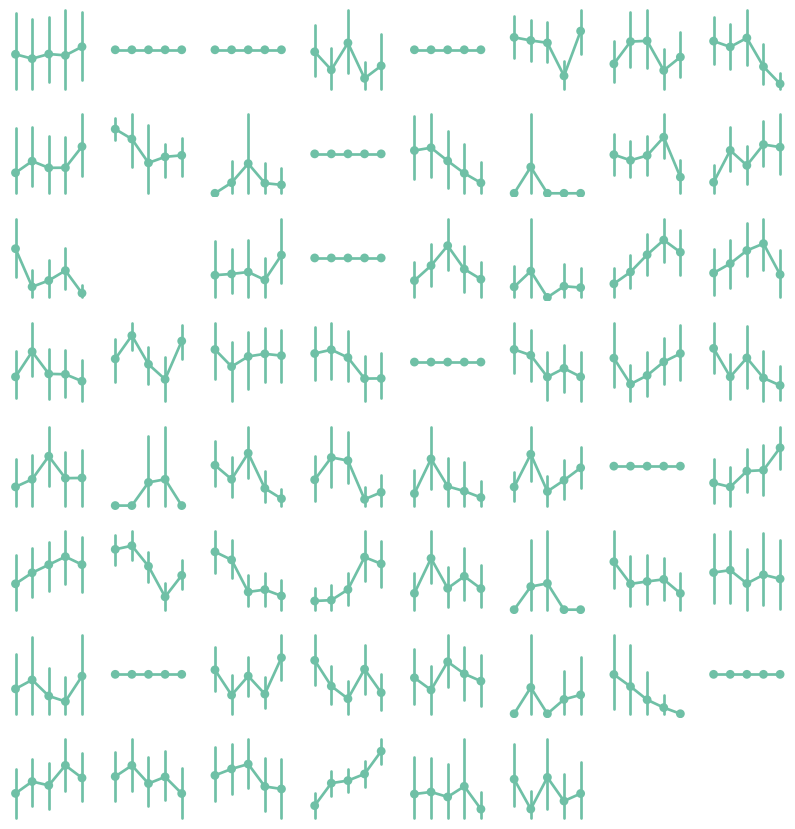
\includegraphics[width=\textwidth]{figures/quantitative/pointplots/clustering_coeff_all.png}
        \caption{Boxplots for normalized clustering coefficient in all repositories mined.}
        \label{app:clustering-box-app}
    \end{figure}

    \begin{figure}[!htb]
        \centering
        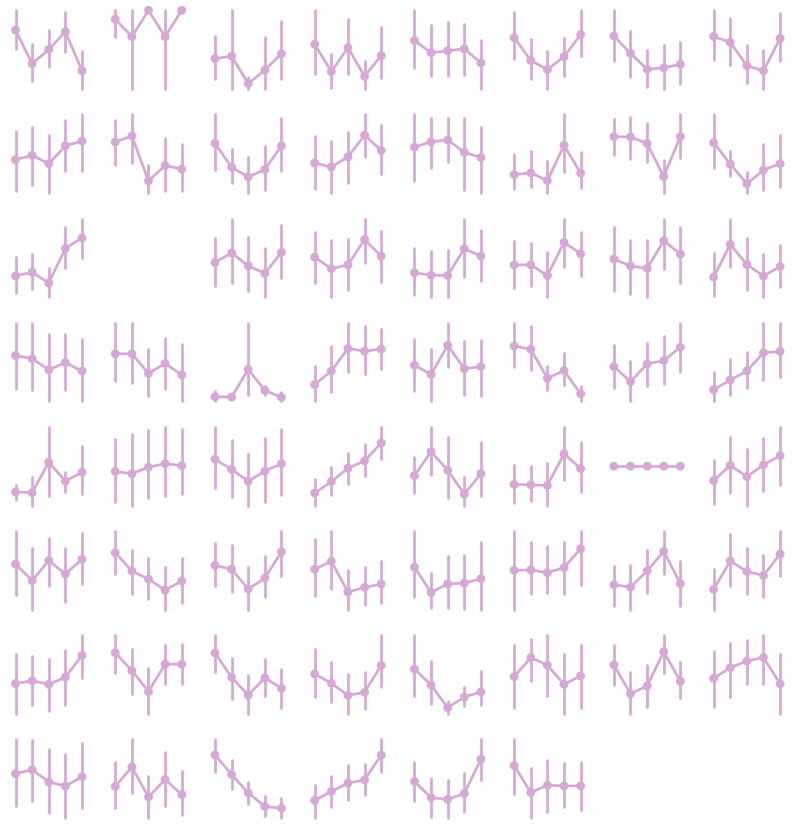
\includegraphics[width=\textwidth]{figures/quantitative/pointplots/cp_ratio_all.png}
        \caption{Boxplots for core-periphery ratio in all repositories mined.}
    \end{figure}

    \begin{figure}[!htb]
        \centering
        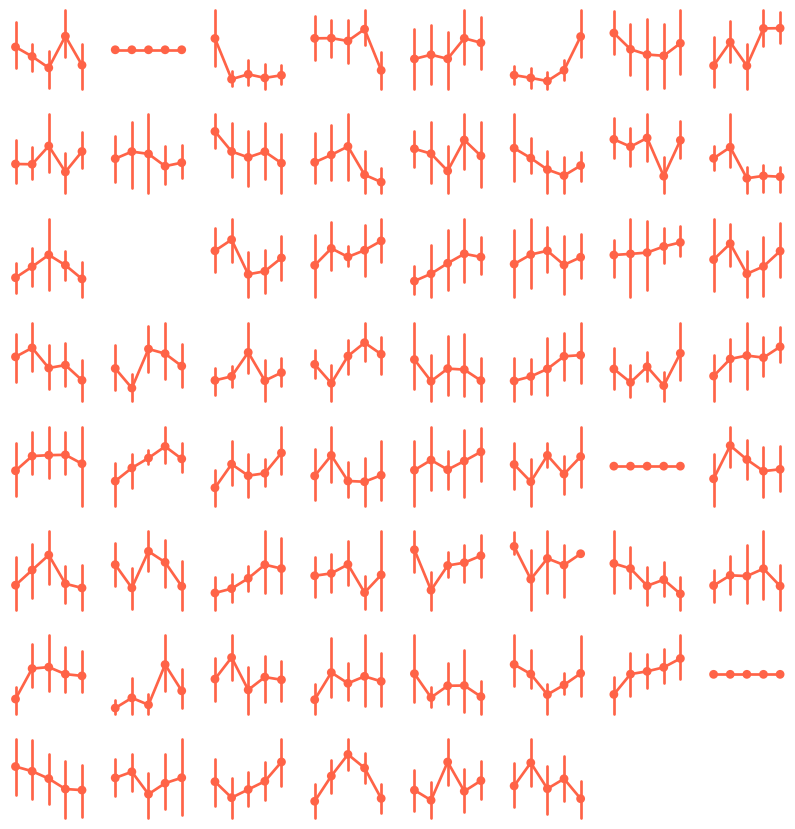
\includegraphics[width=\textwidth]{figures/quantitative/pointplots/hierarchy_all.png}
        \caption{Boxplots for hierarchy in all repositories mined.}
    \end{figure}

\end{appendices}


\end{document}